\documentclass[11pt]{report}

\usepackage{url}
\usepackage{graphicx}
\usepackage{pmboxdraw}
\title{\huge{\Cardpeek{} Reference Manual - v0.5}}
\author{Copyright 2009-2010, L1L1@gmx.com}
%\date{March 2010}
\addtolength{\textwidth}{2cm}
\addtolength{\hoffset}{-1cm}

\newcommand{\mansection}[1]{\vspace{0.5em}\par\noindent\textsc{#1}\vspace{0.5em}\par}
\newcommand{\syn}[1]{\texttt{#1}}
\newcommand{\Cardpeek}{\textsc{Cardpeek}}

\begin{document}
\maketitle

\chapter*{Presentation}

\Cardpeek{} is a program that reads the contents of smart cards. 
This GNU/Linux tool has a GTK GUI and can be extended with the LUA programming language. 
It requires a PCSC card reader to communicate with a smart card.

Smartcards are becoming ubiquitous in our everyday life. 
We use them for payment, transport, in mobile telephones and many other applications.
These cards often contain a lot of personal information such as, for example, our last purchases or 
our last journeys in public transport.

\Cardpeek's goal is to allow you to access all this personal information. As such, you 
can be better informed about the data that is collected about you.

\Cardpeek{} explores ISO 7816 compliant smart cards and represents their content in an organized 
tree format that roughly follows the structure it has inside the card, which is also similar to a 
classical file-system structure.

In this version, this tool is capable of reading the contents of the following types of cards:
\begin{itemize}
\item{EMV "chip and PIN" bank cards used in many countries throughout the world;}
\item{Electronic/Biometric passports, which have an embedded contacless chip (a contactless reader is required);}
\item{\textit{Navigo} transport cards used in Paris and other \textit{Calypso} cards used in France and elsewhere;}
\item{Moneo, the French electronic purse (with limited data interpretation);}
\item{Vitale 2, the French health card.}
\end{itemize}

Some important card types are missing such as the SIM card used in mobile phones.
However, this application can be modified and extended easily to your needs with the embedded LUA scripting language.

For more information on the LUA project see \url{http://www.lua.org/}.

This software has been tested with traditional PCSC card readers (such as the Gemalto\texttrademark PC TWIN) 
as well as contactless or dual-interface PCSC readers (such as the Omnikey\texttrademark 5321). 
Support for the ACG\texttrademark Multi-ISO contactless card reader is still experimental but has been 
reported to work well for traditional ISO 7816 compliant cards.

\tableofcontents

%%%%%%%%%%%%%%%%%%%%%%%%%%%%%%%%%%%%%%%%%%%%%%%%%%%%%%%%%%%%%%%%%%%%%%%%%%%%%%%%%%%%%%%%%%%%%%%%%%
\chapter{Installation}
%%%%%%%%%%%%%%%%%%%%%%%%%%%%%%%%%%%%%%%%%%%%%%%%%%%%%%%%%%%%%%%%%%%%%%%%%%%%%%%%%%%%%%%%%%%%%%%%%%

\Cardpeek{} can be compiled from source using the provided \texttt{Makefile}.
It has currently been tested under \emph{Linux Debian version 5} (both i386 and amd64).

It has been reported to compile and work under \emph{FreeBSD} as well, with a minor tweak.

Note that, in most cases, cryptography export control restrictions do not apply to the source code
of \Cardpeek: all cryptographic operations are implemented in the external \texttt{openssl} 
library.

%-%-%-%-%-%-%-%-%-%-%-%-%-%-%-%-%-%-%-%-%-%-%-%-%-%-%-%-%-%-%-%-%-%-%-%-%
\section{Compiling and installing}

Instructions:
\begin{enumerate}
\item{Make sure you have the following development packages installed:
  \begin{itemize}
  \item{libgtk 2.0 (\url{http://www.gtk.org})}
  \item{liblua 5.1 (\url{http://www.lua.org})}
  \item{libpcsclite (\url{http://pcsclite.alioth.debian.org/})}
  \item{libssl (\url{http://www.openssl.org/})}
  \end{itemize}
(Note: On a Debian system, these packages are all available through \texttt{apt}/\texttt{aptitude}.)}
\item{Unpack the source if needed and change directory to the source directory.}
\item{Type\footnote{Note for FreeBSD: before executing \texttt{make}, 
you will need to make a small change in the Makefile included in the source, 
as described in the comments included in that file.} `\texttt{make}'}
\item{The binary executable is `\texttt{cardpeek}', use it directly or copy it to the desired location.}
\end{enumerate}


%-%-%-%-%-%-%-%-%-%-%-%-%-%-%-%-%-%-%-%-%-%-%-%-%-%-%-%-%-%-%-%-%-%-%-%-%
\section{Related files and initial setup}
The first time \Cardpeek{} is run, it will attempt to create the
\texttt{.cardpeek/} directory in your home directory. This is normal.

The \texttt{.cardpeek/} directory will contain two elements: \texttt{config.lua} and the \texttt{scripts/} directory.
The \texttt{config.lua} allows you to run commands automatically when the program starts 
(it should become a full fledged `config file' in the future).
The \texttt{scripts/} directory contains all the scripts that allow to explore smart cards. 
Currently it contains 7 LUA files: ``\texttt{emv.lua}'', ``\texttt{navigo.lua}'', ``\texttt{calypso.lua}'', 
``\texttt{moneo.lua}'', ``\texttt{vitale\_2.lua}'', ``\texttt{e-passport.lua}'' and ``\texttt{atr.lua}''.
These files all show up in the `analyzer' menu of \Cardpeek{} (without their extension `.lua').
If you add any LUA file to this directory, it will thus also appear in the menu.
The \texttt{scripts/} directory contains a subdirectory \texttt{lib/} that holds a few LUA files containing 
frequently used commands that are shared among the card processing scripts.

Each time the program runs, it creates a file \texttt{.cardpeek.log} in your home directory.
This file contains a copy of the messages displayed in the ``log'' tab of the application (see next chapter). 

%%%%%%%%%%%%%%%%%%%%%%%%%%%%%%%%%%%%%%%%%%%%%%%%%%%%%%%%%%%%%%%%%%%%%%%%%%%%%%%%%%%%%%%%%%%%%%%%%%
\chapter{Using Cardpeek}
%%%%%%%%%%%%%%%%%%%%%%%%%%%%%%%%%%%%%%%%%%%%%%%%%%%%%%%%%%%%%%%%%%%%%%%%%%%%%%%%%%%%%%%%%%%%%%%%%%

%-%-%-%-%-%-%-%-%-%-%-%-%-%-%-%-%-%-%-%-%-%-%-%-%-%-%-%-%-%-%-%-%-%-%-%-%
\section{Quick start}

To experiment with \Cardpeek, your may start with your EMV ``PIN and chip'' smart card for example, 
by following these steps:
\begin{enumerate}
\item{Start \texttt{cardpeek}.}
\item{Select your PCSC card reader in the first dialog box.}
\item{Insert your EMV ``PIN and chip'' card in the card reader.}
\item{Select \emph{emv} in the \emph{analyzer} menu. This will run the default \emph{emv} script.}
\item{View the results in the ``card data'' tab.}
\end{enumerate}

On many bank cards, you will discover a surprising amount of transaction log data (look at the ``log data'' 
in the displayed card data).

%-%-%-%-%-%-%-%-%-%-%-%-%-%-%-%-%-%-%-%-%-%-%-%-%-%-%-%-%-%-%-%-%-%-%-%-%
\section{User interface}

The user interface is divided in four main parts: 3 tabs and a one-line command input field.

\begin{center}
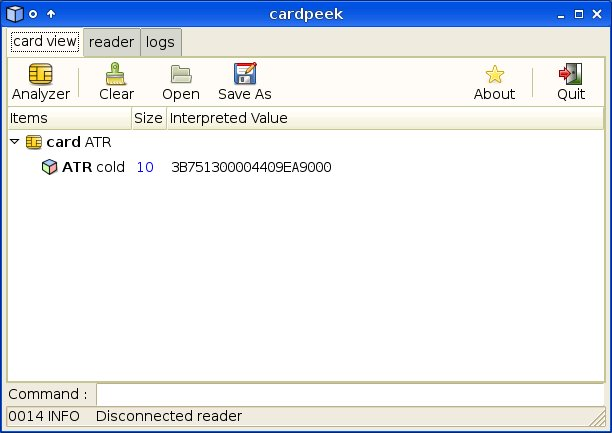
\includegraphics[width=.75\textwidth]{graphics/sample-blank.jpg}
\end{center}

Each one of the 3 tabs proposes a different view of card related information:
\begin{description}
\item[`card view']{shows card data extracted from a card in a structured \emph{tree} form.}  
\item[`reader']{shows raw binary data exchanged between the host PC and the card reader.}
\item[`log']{displays a journal of application events, mainly usefull for debugging purposes.}  
\end{description}

\subsection{card view}

The \emph{card view} tab is the central user interface component of \Cardpeek. 

It represents the data extracted from a card in a structured \emph{tree} from.
This tree structure is initially blank and is entirely constructed by the LUA scripts that are executed (see next chapter).
This tree can be saved and loaded in XML format (see \ref{section:xmlformat}) using the commands in the \emph{data} menu.

The \emph{card view} tab offers the following action buttons:

\vspace{1em}\noindent
\begin{tabular}{l|p{12cm}}
\hline
\emph{Analyse}    & Clicking on this button spawns a menu from which an card analysis script can be chosen (see next chapter). \\  
\hline
\emph{Clear}      & This button clears the card tree view.\\
\hline
\emph{Open}       & This button allows to load a previously saved card tree representation from an XML file.\\
\hline
\emph{Save As}    & This button allows to save the current card tree representation into an XML file. \\
\hline
\emph{About}      & This button displays a very brief message about \Cardpeek. \\
\hline
\emph{Quit}       & This button quits the application. \\
\hline
\end{tabular}
\vspace{2em}

The \emph{card view} data is represented in 3 columns. The first column displays the nodes of the card tree view
in a hierarchical structure similar to a typical file directory tree browser. The second column displays the size
of the node data (most frequently expressed in bytes). Finally, the third column displays the node data itself.
The node data can either be represented in ``raw'' (hexadecimal) form or in a more user friendly ``alternative'' form
(such as a text, or a date).
By default, the tree view will display node data in a user friendly ``alternative'' format if it exists. 
By clicking on the column title, it is possible to switch between both ``raw'' and ``alternative'' data representations.

When node data is over 128 bytes in size, it is truncated for display in the card view window. 
This indicated by appending \textbf{[...]} to the truncated data. By double-clicking on the data, it is possible
to switch to the full representation of the node data.

\subsection{The reader tab}

The reader tab displays the raw binary data exchanges between the card reader and the card itself. 
This data is mainly composed of command APDUs and card responses. Command APDUs are represented by a single
block of data, while card responses contain two elements: a card status word and card response data.

One interesting feature of the card reader tab is the ability to save the APDU/response exchanges between the card reader and
the card in a file that can later be used to emulate the card. Once card this data is saved in a file (with the .clf
extension) and placed in the \syn{.cardpeek/log/} folder, it will appear as a choice in the card reader selection
window that appear when \texttt{cardpeek} is launched. The name of the file will be prefixed by 
``\url{emulator://}'' in the card selection window. Selecting such a card data file allows to re-run the script
on the previously recorded APDU/response data instead of a real card inserted in the card reader. This is very useful for
testing and debugging card scripts without relying on a real card inserted in the card reader.

The \emph{reader} tab offers the following action buttons:

\vspace{1em}\noindent
\begin{tabular}{l|p{12cm}}
\hline
\emph{Connect}    & This button establishes a connexion between the card and the card reader. \\  
\hline
\emph{Reset}      & This button performs a warm reset of the card.\\
\hline
\emph{Disconnect} & This button closes the connexion between the card and the card reader.\\
\hline
\emph{Clear}      & This button clears the APDU/response data displayed in the window. \\
\hline
\emph{Save as}     & This button allows to save the displayed APDU/response data, either for future examination or
		     to be replayed as an emulation of a real card. \\
\hline
\end{tabular}
\vspace{2em}

``Connect'', ``Reset'' and ``Disconnect'' operations are usually automatically done by the card scripts.
However, it is occasionally practical to manually force the execution of these commands.

\subsection{The log tab}

The \emph{log} tab keeps track of \emph{messages} emitted by the application or the script being run.
These messages are useful for monitoring and for debugging purposes. 
The last message also appears at the bottom of the screen in the status bar.

\subsection{The one-line command input field}

The one-line \emph{command} input field at the bottom of the window allows to type single LUA commands that will be 
directly executed by the application.
This is useful for testing some ideas quickly or for debugging purposes.

%-%-%-%-%-%-%-%-%-%-%-%-%-%-%-%-%-%-%-%-%-%-%-%-%-%-%-%-%-%-%-%-%-%-%-%-%
\section{Card-reader selection}

When the program starts, you'll be asked to choose a card reader. 
This will give you 3 main choices :
\begin{enumerate}
\item{\emph{Select a PCSC card reader to use:}
  You may have several of PCSC card readers attached to your computer.
      	  Card-readers are usually identified by their name, preceded by \url{pcsc://}.}
\item{\emph{Select a file containing previously recorded card APDU/response data:}
  This allows to emulate a smart card that was previously in the reader, and is quite convenient
  for script debugging purposes.
  Each time an APDU is sent to the emulated card, \Cardpeek{} will answer with the previously 
  recorded response data (or return an error if the query is new).
  Files containing previously recorded APDU/response data are identified by a file name, preceded by 
  \url{emulator://}.}
\item{\emph{Select ``none'':}
  Selecting \texttt{none} is useful if you do not wish to use a card reader at all, for example if 
  you only want to load and examine card data that was previously saved in XML format.}
\end{enumerate}

%%%%%%%%%%%%%%%%%%%%%%%%%%%%%%%%%%%%%%%%%%%%%%%%%%%%%%%%%%%%%%%%%%%%%%%%%%%%%%%%%%%%%%%%%%%%%%%%%%
\chapter{Card analysis tools}
%%%%%%%%%%%%%%%%%%%%%%%%%%%%%%%%%%%%%%%%%%%%%%%%%%%%%%%%%%%%%%%%%%%%%%%%%%%%%%%%%%%%%%%%%%%%%%%%%%

\begin{center}
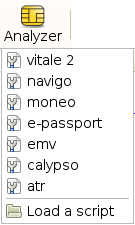
\includegraphics[width=.25\textwidth]{graphics/sample-menu-analyzer.png}
\end{center}

Cardpeek provides several card analysis tools, which all appear in the "Analyzer" menu. 
These tools are actually ``scripts'' written in the LUA language, and \Cardpeek{} allows you to 
add your own scripts easily.
As described in chapter \ref{chapter:licence}, these scripts are provided WITHOUT ANY WARRANTY.

%-%-%-%-%-%-%-%-%-%-%-%-%-%-%-%-%-%-%-%-%-%-%-%-%-%-%-%-%-%-%-%-%-%-%-%-%
\section{atr}

\paragraph{Overview:}
This script simply prints the ATR (Answer To Reset) of the card.

\paragraph{Notes:}
In the future this script will be enhanced with a detailed analysis of the ATR.

%-%-%-%-%-%-%-%-%-%-%-%-%-%-%-%-%-%-%-%-%-%-%-%-%-%-%-%-%-%-%-%-%-%-%-%-%
\section{calypso}

\paragraph{Overview:}
This script provides an analysis of Calypso public transport cards used in many cities.

\paragraph{Notes:}
You will notice that many of these transport cards keep a ``event log'' describing at least 3 of the last stations/stops you have been through.
This ``event log'', which could pose a privacy risk, is not protected by any access control means and is freely readable.

%-%-%-%-%-%-%-%-%-%-%-%-%-%-%-%-%-%-%-%-%-%-%-%-%-%-%-%-%-%-%-%-%-%-%-%-%
\section{emv}

\begin{center}
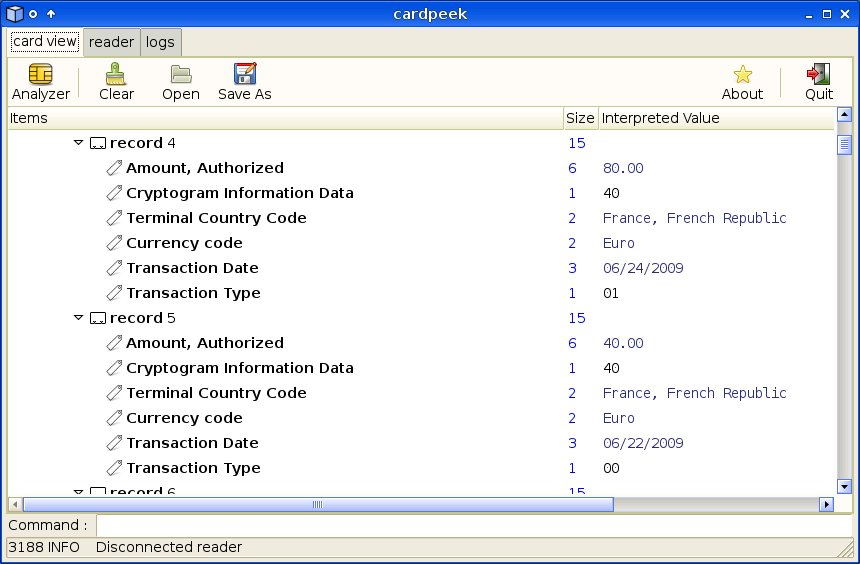
\includegraphics[width=1\textwidth]{graphics/sample-emv.jpg}
\end{center}

\paragraph{Overview:}
This script provides an analysis of EMV banking cards used across the world.

\paragraph{Notes:}
This script will ask you if you want to issue a \emph{Get Processing Option} (GPO) command for each application on the card.
Since some cards have several applications (e.g. a national and an international application), this question may be asked twice or more.
This command is needed to allow access to some information in the card.
Issuing this command will also increase an internal counter inside the card (the ATC). 

You will notice that many of these bank cards keep a ``transaction log'' of the last transactions you have made with your card.
Some banks cards keep way over a hundred transactions that are freely readable, which brings up some privacy issues.

%-%-%-%-%-%-%-%-%-%-%-%-%-%-%-%-%-%-%-%-%-%-%-%-%-%-%-%-%-%-%-%-%-%-%-%-%
\section{e-passport}

\begin{center}
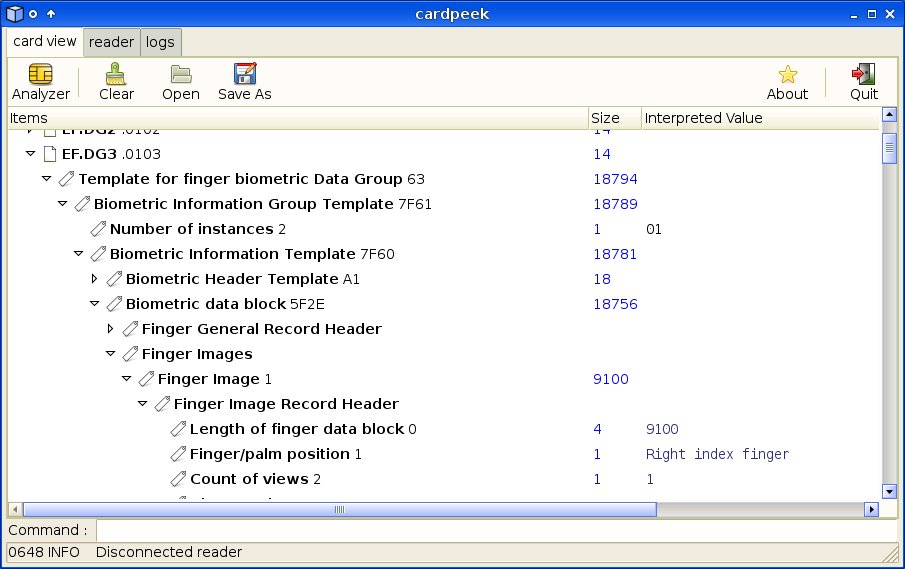
\includegraphics[width=1\textwidth]{graphics/sample-epassport.jpg}
\end{center}

\paragraph{Overview:}
This script provides an analysis of data in a electronic/biometric passport, through a contactless interface.

\paragraph{Notes:}
This script implements the BAC (Basic Access Control) secure access algorithm to access data in the passport. 
It will not be able to access data protected with the EAC (Enhances Access Control) algorithm.
When the script starts, you will be required to input the lower part of the MRZ (Machine Readable Zone) data on the passport. 
This data is needed to compute the cryptographic keys used in the BAC algorithm.

This scripts attempts to parse biometric facial and fingerprint image data.

%-%-%-%-%-%-%-%-%-%-%-%-%-%-%-%-%-%-%-%-%-%-%-%-%-%-%-%-%-%-%-%-%-%-%-%-%
\section{moneo}

\paragraph{Overview:}
This scripts provide a (limited) analysis of MONEO electronic purse cards used in France.

\paragraph{Notes:}
The provided output is very "raw".

%-%-%-%-%-%-%-%-%-%-%-%-%-%-%-%-%-%-%-%-%-%-%-%-%-%-%-%-%-%-%-%-%-%-%-%-%
\section{navigo}

\begin{center}
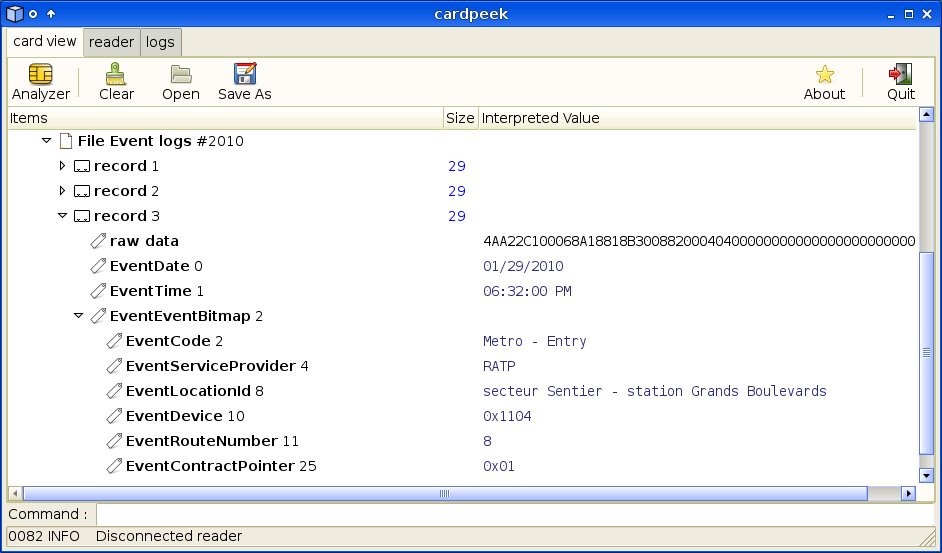
\includegraphics[width=1\textwidth]{graphics/sample-navigo.jpg}
\end{center}

\paragraph{Overview:}
This script is a specialized version of the \texttt{calypso} script, specifically targeted for the Navigo cards used in Paris.
It provides enhanced ``event log'' analysis notably with subway/train station names, as illustrated in the example above.
It has been successfully tested on \emph{Navigo D\'ecouverte}, \emph{Navigo} and \emph{Navigo Int\'egrale} cards.

\paragraph{Notes:}
You must use the contact interface to read a Navigo card, because they cannot be read with a normal contactless 
card reader (these cards use a specific protocol that is not fully compatible with ISO 14443 B).
See the section about \emph{calypso} for other information.

%-%-%-%-%-%-%-%-%-%-%-%-%-%-%-%-%-%-%-%-%-%-%-%-%-%-%-%-%-%-%-%-%-%-%-%-%
\section{vitale 2}

\paragraph{Overview:}
This script provides an analysis of the second generation French health card called ``Vitale 2''.

\paragraph{Notes:}
This analysis is based on a lot of guesswork and needs further testing.
Some zones, notably the one containing the cardholder's photography, seem protected: this is a good design choice in terms of privacy protection.

%-%-%-%-%-%-%-%-%-%-%-%-%-%-%-%-%-%-%-%-%-%-%-%-%-%-%-%-%-%-%-%-%-%-%-%-%
\section{Adding your own scripts to Cardpeek}
Adding or modifying a script in \Cardpeek{} is easy: simply add or modify a script in the \texttt{\$HOME/.cardpeek/scripts/} directory.

If you want to go further and make a script permanently part of the source code of \Cardpeek, you should follow these additional steps:
\begin{enumerate}
\item{Go to the directory containing the source code of \Cardpeek.}
\item{Execute the \texttt{update\_dot\_cardpeek\_dir.sh} script (e.g. type ``\texttt{. update\_do\_cardpeek.sh}'')}
\item{Run \texttt{make} to rebuild \Cardpeek.}
\end{enumerate}

%%%%%%%%%%%%%%%%%%%%%%%%%%%%%%%%%%%%%%%%%%%%%%%%%%%%%%%%%%%%%%%%%%%%%%%%%%%%%%%%%%%%%%%%%%%%%%%%%%
\chapter{Script language description}
%%%%%%%%%%%%%%%%%%%%%%%%%%%%%%%%%%%%%%%%%%%%%%%%%%%%%%%%%%%%%%%%%%%%%%%%%%%%%%%%%%%%%%%%%%%%%%%%%%

The individual scripts that allow to process different types of smart cards are located in your 
\texttt{\$HOME/.cardpeek/scripts/} directory.
These scripts are written in LUA, a programming language which shares some similarities with Pascal and Javascript.
To allow LUA scripts to communicate with smart cards and to manipulate card data, the LUA language was extended with custom libraries.
This section first starts with a brief example of the script language and then describes the library extensions.

%-%-%-%-%-%-%-%-%-%-%-%-%-%-%-%-%-%-%-%-%-%-%-%-%-%-%-%-%-%-%-%-%-%-%-%-%
\section{Introductory examples}

Here's a short LUA script that demonstrates how to get and print the ATR (Answer To Reset) of a card to the console.

\begin{verbatim}
     card.connect()
     print(card.last_atr())
     card.disconnect()
\end{verbatim}

Next, here's (a slightly longer) script that performs a similar task, while presenting the results using \Cardpeek's user interface instead of the console. 

\begin{verbatim}
     card.connect()

     atr = card.last_atr()

     if atr then
        mycard = ui.tree_add_node(nil,"card")
        ref = ui.tree_add_node(mycard,"ATR","cold")
        ui.tree_set_value(ref,atr)
     end

     card.diconnect()
\end{verbatim}

The fist command \syn{card.connect()} powers-up the card in the card reader and prepares the card for communication. 
Next \syn{card.last\_atr()} returns the ATR of the card. 
If the value of the ATR is non-nil, the script creates a node called ``card'' (with \syn{ui.tree\_add\_node()}). 
This node will appear at the root of the card data tree-view.
A child node called ``ATR'' is added to the root ``card'' node. 
The hexadecimal value of the ATR is associated with the child node.
Finally, the card is powered down with the \syn{card.disconnect()} function.

The final output of the script should have roughly the following structure:

\vspace{2ex}
\begin{tabular}{ll}
$\triangleright$ \textbf{card}&\\
\hspace{1em}\textSFii\textbf{ATR} cold &\texttt{3B6F0000805A0803040002002531F405909000}\\
\end{tabular}
\vspace{2ex}

The example above is equivalent to the ``atr'' script provided with \Cardpeek.
The LUA language is easy to learn and we refer the reader to \url{http://www.lua.org/} for more information.

%-%-%-%-%-%-%-%-%-%-%-%-%-%-%-%-%-%-%-%-%-%-%-%-%-%-%-%-%-%-%-%-%-%-%-%-%
\section{the \syn{bit} library}

Since LUA does not have native bit manipulation functions, the following functions have been added.

%------------------------------------------------
\subsection{bit.AND}

\mansection{Synopsis}
\syn{bit.AND(A,B)}

\mansection{Description}
Compute the binary operation \syn{A} \textit{and} \syn{B}.

%------------------------------------------------
\subsection{bit.OR}

\mansection{Synopsis}
\syn{bit.OR(A,B)}

\mansection{Description}
Compute the binary operation \syn{A} \textit{or} \syn{B}.

%------------------------------------------------
\subsection{bit.XOR}

\mansection{Synopsis}
\syn{bit.XOR(A,B)}

\mansection{Description}
  Compute the binary operation \syn{A} \textit{xor} \syn{B}.

%------------------------------------------------
\subsection{bit.SHL}

\mansection{Synopsis}
\syn{bit.SHL(A,B)}

\mansection{Description}
  Shift the bits of A by B positions to the left. 
  This is equivalent to computing $\syn{A}{\times}2^{\syn{B}}$.

%------------------------------------------------
\subsection{bit.SHR}

\mansection{Synopsis}
\syn{bit.SHR(A,B)}

\mansection{Description}
  Shift the bits of A by B positions to the right. 
  This is equivalent to computing $\syn{A}/2^{\syn{B}}$

%-%-%-%-%-%-%-%-%-%-%-%-%-%-%-%-%-%-%-%-%-%-%-%-%-%-%-%-%-%-%-%-%-%-%-%-%
\section{The \syn{bytes} library}

The \syn{bytes} library provides a new opaque type to LUA: a \textit{bytestring}, 
which is used to represent an array of binary elements. 

Bytestrings are mainly used to represent binary data exchanged with
the card reader in the application.

The elements in the array are most commonly (8 bit) bytes, but
it is also possible to construct arrays of (4 bit) half-bytes or
arrays of individual bits. All elements in a bytestring have the same
size (8, 4 or 1), which is referred as the ``\emph{width}'' of the bytestring.
The width of each element is specified when the array is created 
with the function \syn{bytes.new()} described in this section. 
A function to convert between bytestrings of different widths 
is also provided.

Individual elements in a bytestring array can be accessed the same 
way traditional arrays are accessed in LUA. Thus, if \syn{BS} is
a bytestring the following expressions are valid:

\begin{verbatim}
   BS[0]=1
   print(BS[0])
\end{verbatim} 

Contrary to the LUA tradition, the first index in a bytestring is 0
(instead of 1). The number of elements in a bytestring is indicated 
by prefixing the bytestring with the ``\syn{\#}'' operator, just as 
with an array (e.g. \syn{\#BS}).

Bytestrings cannot be copied like arrays with a simple assignment 
using the ``\syn{=}'' operator, the \syn{bytes.assign()} function
or the \syn{bytes.clone()} function must be used instead.  

The functions of the \syn{bytes} library are next described.

%------------------------------------------------
\subsection{Operators on bytestrings}
  
The operators that can be used on bytestrings are ``\syn{..}'', ``\syn{==}'', ``\syn{$\sim$=}'' and ``\syn{\#}''

\mansection{Synopsis}

\syn{A..B} 

\syn{A==B}

\syn{A$\sim$=B}

\syn{\#A}

\mansection{Description}
  
The ``..'' operator creates a new bytestring by concatenating two bytestrings together.
The concatenation operator also works if one of the operands is a string or a number, 
by converting it to a bytestring first, following the rules described in the 
\syn{bytes.assign()} function. 
\syn{A..B} is equivalent to \syn{bytes.concat(A,B)}.
  
The ``=='' and ``$\sim$='' operators allow to compare two bytestrings for equality or
non-equality respectively. To be equal, two bytestrings must have the same width
and the same elements in the same order.
 
Finally the ``\#'' operator returns the number of elements in a bytestring.

%------------------------------------------------
\subsection{bytes.append}

\mansection{Synopsis}

\syn{bytes.append(BS, value$_0$ [, value$_1$, ..., value$_n$])}

\mansection{Description}

Append a value to \syn{BS}.

The appended value is composed of \syn{value$_0$}, optionally concatenated with
any additional value \syn{value$_1$}, ..., \syn{value$_n$} (from left to right).

This function is equivalent to 
\syn{bytes.assign(BS, BS, \syn{value$_0$} [, \syn{value$_1$}, ..., \syn{value$_n$}])}.
See \syn{bytes.assign()} for further details.

This function modifies its main argument \syn{BS}.

\mansection{Return value}

This function returns \syn{true} upon success and \syn{false} otherwise.

%------------------------------------------------
\subsection{bytes.assign}

\mansection{Synopsis}
\syn{bytes.assign(BS, \syn{value$_0$} [, \syn{value$_1$}, ..., \syn{value$_n$}])}

\mansection{Description}

  Assigns a value to \syn{BS}. 

  The assigned value is composed of \syn{value$_0$}, optionally concatenated with 
  any additional value \syn{value$_1$}, ..., \syn{value$_n$} (from left to right).

  Each \syn{value$_i$} can be either a bytestring, a string or a number.
  If \syn{value$_i$} is a bytestring, each element of \syn{value$_i$} is appended to \syn{BS}, 
  without any conversion.

  If \syn{value$_i$} is a string, it is interpreted as a text representation of
  a bytestring (as returned by the \syn{tostring()} operator). This string
  representation is interpreted by taking into consideration the width 
  of elements of \syn{BS} and is appended to \syn{BS}.

  If \syn{value$_i$} is a number, it is converted into a single bytestring element and 
  appended to \syn{BS}.

  This function modifies its main argument \syn{BS}.

\mansection{Return value}

  This function returns \syn{true} upon success and \syn{false} otherwise.

%------------------------------------------------
\subsection{bytes.clone}

\mansection{Synopsis}
\syn{bytes.clone(BS)}

\mansection{Description}
  Creates and returns a copy of \syn{BS}.

\mansection{Return value}
  This function returns \syn{nil} if it fails.

%------------------------------------------------
\subsection{bytes.concat}

\mansection{Synopsis}
\syn{bytes.concat(\syn{value$_0$}, \syn{value$_1$} [,\syn{value$_2$} , ..., \syn{value$_n$}])}

\mansection{Description}
  Returns the concatenation of \syn{value$_0$}, ..., \syn{value$_n$} (from left to right).

  For the rules governing the processing of \syn{value$_0$} ... \syn{value$_n$}, see
  the \syn{bytes.assign()} function above.

\mansection{Return value}
  This function returns a bytestring upon success and \syn{nil} otherwise.

%------------------------------------------------
\subsection{bytes.convert}

\mansection{Synopsis}
\syn{bytes.convert(w,BS)}

\mansection{Description}
  Converts \syn{BS} to a new bytestring where each element has a width \syn{w}.

  Depending on \syn{w}, the elements in the converted bytestring are obtained by either 
  splitting elements of \syn{BS} into several smaller elements in the new bytestring or 
  by grouping several elements of \syn{BS} into a single element in the new bytestring.

  If the conversion requires splitting elements of \syn{BS}, then the original elements will
  be split with the most significant bit(s) first (the most significant bits of each 
  original element of \syn{BS} will have a lower index than the least significant bits). 

  If the conversion requires grouping elements together, \syn{BS} is will first be 
  right-padded with zeros to a size that is a multiple of \syn{w}. Next, new 
  elements are formed by considering elements of \syn{BS} with a lower index as more 
  significant than elements with a higher index.

\mansection{Return value}
  This function returns a new bytestring upon success and \syn{nil} otherwise.

%------------------------------------------------
\subsection{bytes.insert}

\mansection{Synopsis}
\syn{bytes.insert(BS, pos, \syn{value$_0$} [, \syn{value$_1$}, ..., \syn{value$_n$}])}

\mansection{Description}
  Inserts a value in \syn{BS} at index \syn{pos}.

  The elements in \syn{BS} of index 0 to $pos-1$ will remain untouched.
  The elements in \syn{BS} of index \syn{pos} to \syn{\#BS} are pushed to the right
  to make room for the inserted value.

  The inserted value is composed of \syn{value$_0$}, optionally concatenated with
  any additional value \syn{value$_1$}, ..., \syn{value$_n$} (from left to right).

  For the rules governing the processing of \syn{value$_0$} ... \syn{value$_n$}, see
  the \syn{bytes.assign()} function above.

  This function modifies its main argument \syn{BS}.
  
\mansection{Return value}
  This function returns \syn{true} upon success and \syn{false} otherwise.

%------------------------------------------------
\subsection{bytes.invert}

\mansection{Synopsis}
\syn{bytes.invert(BS)}

\mansection{Description}
  Reverses the order of elements in \syn{BS}.

  If \syn{BS} has \syn{N} elements then \syn{BS[0]} is swapped with \syn{BS[N-1]},
  \syn{BS[1]} is swapped with \syn{BS[N-2]} and so forth until all elements are
  in reverse order in \syn{BS}.

  This function modifies its main argument.
\mansection{Return value}
  This function returns \syn{true} upon success and \syn{false} otherwise.


%------------------------------------------------
\subsection{bytes.is\_printable}

\mansection{Synopsis}
\syn{bytes.is\_printable(BS)}

\mansection{Description}
  Returns \syn{true} if all elements in \syn{BS} can be converted to 
  printable ascii characters, and \syn{false} otherwise.

\mansection{Return value}
  This function always returns \syn{false} if the width of \syn{BS} is 
  not 8 (elements of width 4 or 1 are not printable ascii values).  


%------------------------------------------------
\subsection{bytes.maxn}

\mansection{Synopsis}
\syn{bytes.maxn(BS)}

\mansection{Description}
  Returns the last index in \syn{BS} (equivalent to $\#BS-1$).
\mansection{Return value}
  This function returns \syn{nil} if \syn{BS} is empty.


%------------------------------------------------
\subsection{bytes.new}

\mansection{Synopsis}
\syn{bytes.new(width [,\syn{value$_0$}, \syn{value$_1$}, ..., \syn{value$_n$}])}

\mansection{Description}
  Creates a new bytestring, where each element is \syn{width} bits in size.
  \syn{width} can be either 8, 4 or 1.

  A value can optionally be assigned to the bytestring by specifying one or 
  several values \syn{value$_0$}, \syn{value$_1$}, ..., \syn{value$_n$} that will be concatenated
  together to form the content of the bytestring. See the function 
  \syn{bytes.assign()} for more details.
\mansection{Return value}
  This function returns a bytestring upon success and \syn{nil} otherwise. 


%------------------------------------------------
\subsection{bytes.pad\_left}

\mansection{Synopsis}
\syn{bytes.pad\_left(BS, length, value)}

\mansection{Description}
  Pads \syn{BS} on the left with the element \syn{value} until the number of elements 
  of \syn{BS} reaches a multiple of \syn{length}.

  If the size of \syn{BS} is already a multiple of \syn{length}, \syn{BS} is left untouched.

  This function modifies its main argument \syn{BS}.
  
\mansection{Return value}
  This function returns \syn{true} upon success and \syn{false} otherwise.


%------------------------------------------------
\subsection{bytes.pad\_right}

\mansection{Synopsis}
\syn{bytes.pad\_right(BS, length, value)}

\mansection{Description}
  Pads \syn{BS} on the right with the element \syn{value} until the number of elements 
  of \syn{BS} reaches a multiple of \syn{length}.

  If the size of \syn{BS} is already a multiple of \syn{length}, \syn{BS} is left untouched.

  This function modifies its main argument \syn{BS}.
  
\mansection{Return value}
  This function returns \syn{true} upon success and \syn{false} otherwise.


%------------------------------------------------
\subsection{bytes.remove}

\mansection{Synopsis}
\syn{bytes.remove(BS, start [,end])}

\mansection{Description}
  Deletes a part of \syn{BS}.

  Removes all elements of \syn{BS} that have an $index$ that verifies 
  $index \geq \syn{start}$ and $index \leq \syn{end}$.

  The elements in \syn{BS} are re-indexed: \syn{BS[end+1]} becomes \syn{BS[start]},
  \syn{BS[end+2]} becomes \syn{BS[start+1]}, and so forth.

  If \syn{end} is not specified it will default to the last index of \syn{BS}.
  \syn{start} and \syn{end} may be negative to refer to the position of an element by 
  starting from the end of the bytetring as described in \syn{bytes.sub()}.

  This function modifies its main argument \syn{BS}.
  
\mansection{Return value}
  This function returns \syn{true} upon success and \syn{false} otherwise.


%------------------------------------------------
\subsection{bytes.sub}

\mansection{Synopsis}
\syn{bytes.sub(BS, start [,end])}

\mansection{Description}
  Returns a copy of a substring from \syn{BS}.

  The returned value represents a bytestring containing a copy of all the 
  elements of \syn{BS} that have an index that verifies $index \geq \syn{start}$ and 
  $index \leq \syn{end}$.
  If \syn{end} is not specified it will default to the last index of \syn{BS}.
  If \syn{start} (or \syn{end}) is negative, it will be replaced by \syn{\#BS+start}
  (or \syn{\#BS+end} resp.).

\mansection{Return value}
  This function returns a bytestring upon success and \syn{nil} otherwise.


%------------------------------------------------
\subsection{bytes.tonumber}

\mansection{Synopsis}
\syn{bytes.tonumber(BS)}

\mansection{Description}
  Converts the bytestring \syn{BS} to a string representing the unsigned 
  decimal value of \syn{BS}.

  This conversion considers \syn{BS[0]} as the most significant element of \syn{BS}, 
  and \syn{BS[\#BS-1]} as the least significant. 
  
\mansection{Return value}
  This function returns a string.
  If needed LUA will automatically convert the resulting string to a number.


%------------------------------------------------
\subsection{bytes.toprintable}

\mansection{Synopsis}
\syn{bytes.toprintable(BS)}

\mansection{Description}
  Converts each element in \syn{BS} into an ascii character and returns the
  resulting string.

  If an element in \syn{BS} cannot be converted to a printable character it
  is replaced by the character ``?''. 

  If \syn{BS} is empty, the resulting string is also empty.

\mansection{Return value}
  A string.


%------------------------------------------------
\subsection{bytes.width}

\mansection{Synopsis}
\syn{bytes.width(BS)}

\mansection{Description}
  Return the width of the elements in \syn{BS}.

\mansection{Return value}
  This function may return 1, 4 or 8.


%-%-%-%-%-%-%-%-%-%-%-%-%-%-%-%-%-%-%-%-%-%-%-%-%-%-%-%-%-%-%-%-%-%-%-%-%
\section{The \syn{asn1} library}

The ASN1 library allows to manipulate ASN1 TLV bytestrings following the DER/BER 
encoding rules (Distinguished/Basic Encoding Rules).
These bytestrings must be 8 bit wide.

The library provides the following functions.


%------------------------------------------------
\subsection{asn1.enable\_single\_byte\_length}

\mansection{Synopsis}
\syn{asn1.enable\_single\_byte\_length(enable)}

\mansection{Description}
  This function is only used in rare cases with erroneous card implementations.
  
  If $\syn{enable}=true$ the behavior of TLV decoding functions 
  (such as \syn{bytes.tlv\_split()}) are modified by forcing the ASN1 
  length to be 1 byte long. 
  
  This means that even if the first byte of the encoded length is greater 
  than \syn{0x80} it will be interpreted as the length of the TLV value.

\mansection{Return value}
  None.

%------------------------------------------------
\subsection{asn1.join}

\mansection{Synopsis}
\syn{asn1.join(tag, val [,extra])}

\mansection{Description}
  Performs the opposite of \syn{bytes.tlv\_split}: creates a bytestring 
  representing the ASN1 DER encoding of the TLV \{\syn{tag}, \textit{len} , \syn{val}\} where \textit{len}=\syn{\#val} 
  and appends \syn{extra} to the result.

  \syn{tag} is positive integer number, \syn{val} is a bytestring and 
  \syn{extra} is a bytestring or \syn{nil}.

\mansection{Return value}
  This function returns a bytestring.

%------------------------------------------------
\subsection{asn1.split}

\mansection{Synopsis}
\syn{asn1.split(str)}

\mansection{Description}
  Parses the beginning of the bytestring \syn{str} according to ASN1 BER 
  TLV encoding rules, and extracts a tag \syn{T} and a bytestring value \syn{V}.

\mansection{Return value}
  The function returns 3 elements \{\syn{T}, \syn{V}, \textit{extra}\}, 
  where \textit{extra} is an optional bytestring representing the remaining part of 
  \syn{str} that was not parsed or \syn{nil} if no data remains.

  If this function fails it returns a triplet of \syn{nil} values.


%------------------------------------------------
\subsection{asn1.split\_length}

\mansection{Synopsis}
\syn{asn1.split\_length(str)}

\mansection{Description}
  Parses the beginning of the bytestring \syn{str} according to ASN1 BER 
  and extracts a length \syn{L}. 

\mansection{Return value}
  The function returns \{\syn{L}, \textit{extra}\}, where \textit{extra} is an optional bytestring 
  representing the remaining part of \syn{str} that was not parsed or \syn{nil} 
  if no data remains.

  If this function fails it returns a pair of \syn{nil} values.


%------------------------------------------------
\subsection{asn1.split\_tag}

\mansection{Synopsis}
\syn{asn1.split\_tag(str)}

\mansection{Description}
  Parses the beginning of the bytestring \syn{str} according to ASN1 BER 
  and extracts a tag \syn{T}. 

\mansection{Return value}
  The function returns  \{\syn{L}, \textit{extra}\}, where \textit{extra} is an optional bytestring 
  representing the remaining part of \syn{str} that was not parsed or 
  \syn{nil} if no data remains.

  If this function fails it returns a pair of \syn{nil} values.


%-%-%-%-%-%-%-%-%-%-%-%-%-%-%-%-%-%-%-%-%-%-%-%-%-%-%-%-%-%-%-%-%-%-%-%-%
\section{The \syn{card} library}

The \syn{card} library is used to communicate with a smart card in a card reader.

Cardpeek internally defines a minimal set of card functions in the \syn{card} 
library.
Some additional extensions to the \syn{card} library are written in LUA and can
be found in the file \syn{\$HOME/.cardpeek/scripts/lib/apdu.lua}, which should 
be loaded automatically when cardpeek starts.

This library contains the following functions.


%------------------------------------------------
\subsection{card.connect}

\mansection{Synopsis}
\syn{card.connect()}

\mansection{Description}
  Connect to the card currently inserted in the selected smart card reader. 

  This command is used at the start of most smart card scripts.

\mansection{Return value}
   This function returns \syn{true} upon success, and \syn{false} otherwise.


%------------------------------------------------
\subsection{card.disconnect}

\mansection{Synopsis}
\syn{card.disconnect()}

\mansection{Description}
  Disconnect the card currently inserted in the selected smart card reader.
	  
  This command concludes most smart card scripts.

\mansection{Return value}
  This function returns \syn{true} upon success, and \syn{false} otherwise.

%------------------------------------------------
\subsection{card.get\_data}

\mansection{Synopsis}
\syn{card.get\_data(id [, length\_expected])}


\mansection{Description}
  Execute the GET\_DATA command from ISO 7816-4 where:
  \begin{itemize}
  \item{\syn{id} is the tag number of the value to read from the card.}
  \item{\syn{length\_expected} is an optional value specifying the length of the resulting expected result (defaults to 0, which means 256 bytes).}
  \end{itemize}

  The value of ``CLA'' in the command sent to the card is defined by by the variable \syn{card.CLA}.

  This function is implemented in \syn{apdu.lua}.

\mansection{Return value}
  The card status word and response data, as described in \syn{card.send} (section \ref{sec:card_send}).


%------------------------------------------------
\subsection{card.last\_atr}

\mansection{Synopsis}
\syn{card.last\_atr()}

\mansection{Description}
  Returns a bytestring representing the last ATR (Answer To Reset) returned by the card.

\mansection{Return value}
  This function returns a bytestring.

%------------------------------------------------
\subsection{card.make\_file\_path}

\mansection{Synopsis}
\syn{card.make\_file\_path(path)}

\mansection{Description}
  This function is designed to be a helper function for the implementation of \syn{card.select}.

  It converts a human readable path string (representing a file location in
  a smart card) into a format that is compatible with the SELECT\_FILE command from ISO 7816-4.

  This function parses the string \syn{path} and returns a pair of values \{\syn{path\_binary}, \syn{path\_type}\}
  where:
  \begin{itemize}
  \item{\syn{path\_binary} is a bytestring representing the encoded binary value of \syn{path}, and}
  \item{\syn{path\_type} is a number describing the path type (i.e. a relative path, an AID, ...)}
  \end{itemize}

  The general rules needed to form a path string can be summarized as follows:
  \begin{itemize}
  \item{A file ID is represented by 4 hexadecimal digits 
    (however, there is an exception for ADFs that can also be represented by their AID, 
     which requires 10 to 32 hexadecimal digits, or 5 to 16 bytes).}
  \item{If \syn{path} starts with the `\syn{\#}' character, the file is selected directly by its unique ID or AID.}
  \item{If \syn{path} starts with the `\syn{.}' character, the file is selected relatively to the current DF or EF.}
  \item{Files can also be selected by specifying a relative or absolute path, 
    where each element in the path is represented by a 4 digit file ID separated by the `\syn{/}' character:}
     \begin{itemize}
     \item{If \syn{path} starts with `\syn{/}' the file is selected by its full path (excluding the MF).}
     \item{If \syn{path} starts with `\syn{./}' the file is selected by its relative path (excluding the current DF).}
     \end{itemize}
  \end{itemize}

  The next table describes the format of the string \syn{path} and how it is interpreted more precisely. 
  In this table, as a convention, hexadecimal characters are represented with the character `\texttt{h}' 
  and repeated elements are summarized by writing ``[\ldots ]''.

%  \begin{table}[!hbp]
  \vspace{2em}
  \begin{tabular}{|l|p{7cm}|c|}
  \hline
  \syn{path} format 
  & interpretation
  & \syn{path\_type} \\
  \hline
  \hline
  \texttt{\#}
  & Directly select the MF (equivalent to \texttt{\#3F00})
  & 0 \\
  \hline
  \texttt{\#hhhh}
  & Directly select the file with ID=\texttt{hhhh}
  & 0 \\
  \hline
  \texttt{\#hhhhhh}[\ldots ]\texttt{hh}
  & Directly select the DF with AID=\texttt{hhhhhh}[\ldots ]\texttt{hh}    
  & 4 \\
  \hline
  \hline
  \texttt{.hhhh}
  & Under the current DF, select the file with ID=\texttt{hhhh} 
  & 1 \\
  \hline
  \texttt{.hhhh/}
  & Under the current DF, select the DF with ID=\texttt{hhhh}   
  & 2 \\
  \hline
  \texttt{..} 
  & Select the parent of the current EF or DF.
  & 3 \\
  \hline
  \hline
  \texttt{./hhhh/hhhh/hh}[\ldots ]
  & Select a file using a relative path from the current DF. 
    All intermediary DF's are represented by their file ID 
    separated by the `\texttt{/}' character.
  & 9 \\
  \hline
  \texttt{/hhhh/hhhh/hh}[\ldots ] 
  & Select a file with an absolute path from the MF (the MF is omitted) 
    All intermediary DF's are represented by their file ID 
    separated by the `\texttt{/}' character.
   & 8 \\
  \hline
  \end{tabular}
  \vspace{2em}
%  \end{table}
  

  The resulting bytestring \syn{path\_binary} is simply produced from the concatenation 
  of the hexadecimal values in \syn{path} (represented by `\texttt{h}' in the table above.)

\mansection{Return value}
  Upon success this function returns a pair of values consisting of a bytestring and a number.
  Upon failure, this functions returns a pair of \syn{nil} values.


%------------------------------------------------
\subsection{card.read\_binary}

\mansection{Synopsis}
\syn{card.read\_binary(sfi [, address [, length\_expected]])}


\mansection{Description}
  Execute the READ\_BINARY command from ISO 7816-4 where:
  \begin{itemize}
  \item{\syn{sfi} is a number representing a short file identifier ($1 \le \syn{sfi} \le 30$) or the string `.' to refer to the currently selected file.}
  \item{\syn{address} is an optional start address to read data (defaults to 0).}
  \item{\syn{length\_expected} is an optional value specifying the length of the resulting expected result (defaults to 0, which means 256 bytes).}
  \end{itemize}

  The value of ``CLA'' in the command sent to the card is defined by the LUA variable \syn{card.CLA}.

  This function is implemented in \syn{apdu.lua}.

\mansection{Return value}
  The card status word and response data, as described in \syn{card.send} (section \ref{sec:card_send}).


%------------------------------------------------
\subsection{card.read\_record}

\mansection{Synopsis}
\syn{card.read\_record(sfi, r, [, length\_expected])}


\mansection{Description}
  Execute the READ\_RECORD command from ISO 7816-4 where:
  \begin{itemize}
  \item{\syn{sfi} is a number representing a short file identifier ($1 \le \syn{sfi} \le 30$) or the string `.' to refer to the currently selected file.}
  \item{\syn{r} is the record number to read.}
  \item{\syn{length\_expected} is an optional value specifying the length of the resulting expected result (defaults to 0, which means 256 bytes).}
  \end{itemize}

  The value of ``CLA'' in the command sent to the card is defined by the LUA variable \syn{card.CLA}.

  This function is implemented in \syn{apdu.lua}.

\mansection{Return value}
  The card status word and response data, as described in \syn{card.send} (section \ref{sec:card_send}).


%------------------------------------------------
\subsection{card.select}

\mansection{Synopsis}
\syn{card.select(file\_path [, return\_what [, length]])}

\mansection{Description}
  Execute the SELECT\_FILE command from ISO 7816-4 where:
  \begin{itemize}
  \item{\syn{file\_path} is string describing the file to select, according to the format described in \syn{card.make\_file\_path}.}
  \item{\syn{return\_what} is an optional value describing the expected result, as described in the table below (defaults to 0).}
  \item{\syn{length} is an optional value specifying the length of the resulting expected result (defaults to nil).}
  \end{itemize}

  The following constants have been defined for \syn{return\_what} (some can be combined together by addition):

%  \begin{table}[!hbp]
  \vspace{2em}
  \begin{tabular}{|l|c|}
  \hline
  Constant & value \\
  \hline
  card.SELECT\_RETURN\_FIRST      & 0 \\
  card.SELECT\_RETURN\_LAST       & 1 \\
  card.SELECT\_RETURN\_NEXT       & 2 \\
  card.SELECT\_RETURN\_PREVIOUS   & 3 \\
  card.SELECT\_RETURN\_FCI        & 0 \\
  card.SELECT\_RETURN\_FCP        & 4 \\
  card.SELECT\_RETURN\_FMD        & 8 \\
  \hline
  \end{tabular}
  \vspace{2em}
%  \end{table}

  The value of ``CLA'' in the command sent to the card is defined by by the variable \syn{card.CLA}.
  The value of ``P1'' in the command sent to the card corresponds to the file type computed by \syn{card.make\_file\_path}.
  The value of ``P2'' in the command sent to the card corresponds to \syn{return\_what}.

  This function is implemented in \syn{apdu.lua}.

\mansection{Return value}
  The card status word and response data, as described in \syn{card.send} (section \ref{sec:card_send}).


%------------------------------------------------
\subsection{card.send}
\label{sec:card_send}

\mansection{Synopsis}
\syn{card.send(APDU)}

\mansection{Description}
  Sends the command \syn{APDU} to the card. 

\mansection{Return value}
  The function returns a pair of values: a number representing the status word 
  returned by the card (ex. 0x9000) and the response data returned by the card.
  
  Both the command \syn{APDU} and the response data are bytestrings 
  (see the \syn{bytes} library).


%------------------------------------------------
\subsection{card.info}

\mansection{Synopsis}
\syn{card.info()}

\mansection{Description}
  Return detailed information about the state of the card reader.

\mansection{Return value}
  This function returns an associative array of $(name \Rightarrow value)$ pairs.


%------------------------------------------------
\subsection{card.warm\_reset}

\mansection{Synopsis}
\syn{card.warm\_reset()}

\mansection{Description}
  Performs a warm reset of the card 
  (reconnects the card currently inserted in the selected smart card reader).

\mansection{Return value}
  None

%-%-%-%-%-%-%-%-%-%-%-%-%-%-%-%-%-%-%-%-%-%-%-%-%-%-%-%-%-%-%-%-%-%-%-%-%
\section{The \syn{crypto} library}

This library proposes a limited number of cryptographic functions.
Currently these functions offer mainly DES, Triple-DES, and SHA1 based transformations.

%------------------------------------------------
\subsection{crypto.create\_context}

\mansection{Synopsis}
\syn{crypto.create\_context(algorithm [,key])}

\mansection{Description}
  This function creates a cryptographic ``context'' that holds a description of a 
  cryptographic algorithm, along with a (optional) key.
  The created context is later used as a parameter to other generic functions in the \syn{crypto}
  library, such as \syn{crypto.encrypt()}, \syn{crypto.mac()}, \syn{crypto.digest()}, ...

  The first parameter \syn{algorithm} allows to describe the cryptographic algorithm to be used.
  It can currently take the following values :

  \vspace{2em}
  \begin{tabular}{|l|p{8cm}|}
  \hline
  \textbf{Algorithm}                & \textbf{Description} \\
  \hline
  \hline
  \syn{crypto.ALG\_DES\_ECB}        & Simple DES in ECB mode (no IV). \\
  \hline
  \syn{crypto.ALG\_DES\_CBC}        & Simple DES is CBC mode. \\
  \hline
  \syn{crypto.ALG\_DES2\_EDE\_ECB}  & Triple DES with a double length 112 bit key in ECB mode (no IV). \\
  \hline
  \syn{crypto.ALG\_DES2\_EDE\_CBC}  & Triple DES with a double length 112 bit key in CBC mode.  \\
  \hline
  \syn{crypto.ALG\_ISO9797\_M3}     & ISO 9797 MAC method 3 with a 112 bit key: 
                                      a simple DES CBC MAC iteration with triple DES on the final block.\\
  \hline
  \syn{crypto.ALG\_SHA1}            & The SHA1 digest algorithm. \\
  \hline
  \end{tabular}
  \vspace{2em}

  Some of the previous algorithms only operate on data that has been padded
  to a reach a proper size, that is usually a multiple of a defined ``block size''.
  The value of \syn{algorithm} can be used to specify the padding method that is used, 
  by combining (with the `+' operator) one of the following values to the algorithm 
  previously specified:

  \vspace{2em}
  \begin{tabular}{|l|p{8cm}|}
  \hline
  \textbf{Padding method}           & \textbf{Description} \\
  \hline
  \hline
  \syn{crypto.PAD\_ZERO}            & Add 0's if needed to reach block size. \\
  \hline
  \syn{crypto.PAD\_OPT\_80\_ZERO}   & If the size of cleartext is not already a multiple of block size then
                                      add one byte \texttt{0x80} and then 0's, if needed, to reach block 
                                      size. \\
  \hline
  \syn{crypto.PAD\_ISO9797\_P2}     & ISO 9797 padding method 2 (add a mandatory byte \texttt{0x80} and 
                                      pad with optional 0's to reach block size). \\
  \hline
  \end{tabular}
  \vspace{2em}

  The optional bytestring \syn{key} must be used to specify the value of the cryptographic key used for 
  encryption or MAC algorithms. 

\mansection{Return value}
  This function returns a bytestring representing the created context. Programmers should consider the 
  result as an opaque value and should not modify its content. 

%------------------------------------------------
\subsection{crypto.decrypt}

\mansection{Synopsis}
\syn{crypto.decrypt(context, data [, iv])}

\mansection{Description}
Decrypt the bytestring \syn{data}, using the key and algorithm provided in \syn{context}. 

When the decryption algorithm requires a initial vector, it must be specified in \syn{iv}.

All parameters and the return value are 8 bit wide bytestrings.

\mansection{Return value}
This function returns the decrypted data as a bytestring.  

%------------------------------------------------
\subsection{crypto.digest}

\mansection{Synopsis}
\syn{crypto.digest(context, data)}

\mansection{Description}
Compute the digest (also often called a hash) of \syn{data}, using the algorithm provided in \syn{context}.

All parameters and the return value are 8 bit wide bytestrings.

\mansection{Return value}
This function returns the digest value as a bytestring.

%------------------------------------------------
\subsection{crypto.encrypt}

\mansection{Synopsis}
\syn{crypto.encrypt(context, data [, iv])}

\mansection{Description}
Encrypt the bytestring \syn{data}, using the key and algorithm provided in \syn{context}. 

When the encryption algorithm requires a initial vector, it must be specified in \syn{iv}.

All parameters and the return value are 8 bit wide bytestrings.

\mansection{Return value}
This function returns the encrypted data as a bytestring.

%------------------------------------------------
\subsection{crypto.mac}

\mansection{Synopsis}
\syn{crypto.mac(context, data)}

\mansection{Description}
Computes the MAC (Message Authentication Code) of \syn{data}, using the key and algorithm provided in \syn{context}.

All parameters and the return value are 8 bit wide bytestrings.

\mansection{Return value}
This function returns the (untruncated) MAC as a bytestring.


%-%-%-%-%-%-%-%-%-%-%-%-%-%-%-%-%-%-%-%-%-%-%-%-%-%-%-%-%-%-%-%-%-%-%-%-%
\section{The \syn{ui} library}

The \syn{ui} library allows to control some elements of the user interface of 
\Cardpeek, and in particular the tree structure representing the data 
extracted from the card.

The functions in this library rely on a value called a `\emph{path}' to identify 
each node in the card data tree represented on the screen.
A \emph{path} is a string that is composed of a list of positive numbers separated 
by a colon\footnote{For programmers familiar with GTK++ 2.0, these are the same 
conventions as in the GTK ``tree model''}. 
Each number represents the position (starting at 0) of a node relatively to its parent.
The \emph{path} ``0:2:1'' represents the second child node of the third child 
node of the first top node, and ``0'' simply represents the first top node.
The detailed value of a \emph{path} is usually not important for the programmer, 
who normally manipulates it as an opaque value. 

The \syn{ui} library functions are described in the following paragraphs.


%------------------------------------------------
\subsection{ui.question}

\mansection{Synopsis}
\syn{ui.question(text, buttons)}

\mansection{Description}
  Asks the user a question requesting him to answer by selecting a response.

  The question is described in the string \syn{text}, while the set of 
  possible answers described in the table \syn{buttons}. 
  Each element in \syn{buttons} is string representing a possible answer.
  
\mansection{Return value}
  Upon success, the function returns the index of the answer selected by the 
  user in the table \syn{buttons} 
  (LUA table indexes are usually numbers greater or equal to 1). 
  
  Upon failure the function returns 0.


%------------------------------------------------
\subsection{ui.readline}

\mansection{Synopsis}
\syn{ui.readline(text [,\syn{len} [,\syn{default}]])}

\mansection{Description}
  Request the user to enter a text string. 

  The user's input can optionally be limited to \syn{len} characters and 
  can hold a predefined value \syn{default}.
  
\mansection{Return value}
  The function returns the user's input upon success and \syn{false} otherwise.


%------------------------------------------------
\subsection{ui.tree\_add\_node}

\mansection{Synopsis}
\syn{ui.tree\_add\_node(path\_to\_parent, name, [\syn{id} [, \syn{length} [,\syn{type}]]])}

\mansection{Description}
  Adds a node in the card tree structure. 

  The new node will be appended to the children of the node identified by the 
  \emph{path} \syn{path\_to\_parent}.
  If \syn{path\_to\_parent} is \syn{nil} the new node will be added at 
  the top level.

  \syn{name} describes the type of data that is represented by the node 
  (such as a ``file'' or a ``date of birth'' for example). 

  \syn{id} is an optional identifier that identifies the node uniquely within 
  a context (such as an application ``AID'' or a ``record number'').

  \syn{length} is an optional value number describing the length of the 
  data element associated to the node.

  \syn{type} is an optional informative string that provides additional 
  information describing the type of data represented by the node. This value
  will affect the choice of the icon that is associated with the node in the 
  displayed card tree structure. 

  The following \syn{type} values are associated with a distinct icon: ``application'', ``block'', ``card'', ``file'' and ``record''.
  
\mansection{Return value}
  Upon success the node returns a string representing the \emph{path} to the 
  newly created node. 
  If the function fails, it returns \syn{nil}.
  Once the node is created with this function, data can be associated to it with the \syn{ui.tree\_set\_value} function.


%------------------------------------------------
\subsection{ui.tree\_delete\_node}

\mansection{Synopsis}
\syn{ui.tree\_delete\_node(path\_to\_node)}

\mansection{Description}
  Deletes the node identified by \syn{path\_to\_node} as well as all its 
  children.

\mansection{Return value}
  The function returns \syn{true} upon success and \syn{false} otherwise.


%------------------------------------------------
\subsection{ui.tree\_find\_node}

\mansection{Synopsis}
\syn{ui.tree\_find\_node(origin, name, id)}

\mansection{Description}
  Searches inside the sub-tree of root \syn{origin} for the first node that has 
  name \syn{name} and/or the id \syn{id}.

  If \syn{name=nil} or \syn{id=nil} they are ignored in the search.

\mansection{Return value}
  If a node is found, the function returns the path to that node otherwise 
  it returns \syn{nil}.

%------------------------------------------------
\subsection{ui.tree\_get\_alt\_value}

\mansection{Synopsis}
\syn{ui.tree\_get\_alt\_value(path\_to\_node)}

\mansection{Description}
  Returns the alternative value associated with the node identified by \syn{path\_to\_parent}, 
  or \syn{nil} if no value is associated with the node or if the function fails.

\mansection{Return value}
  This function returns a string.
 

%------------------------------------------------
\subsection{ui.tree\_get\_node}

\mansection{Synopsis}
\syn{ui.tree\_get\_node(path\_to\_node)}

\mansection{Description}
  Returns an array of 5 elements associated to the node identified by 
  \syn{path\_to\_node}.
 
  These elements are: ${name, id, length, comment, num\_children}$. 
  The first 4 elements are the same as the parameters of the function 
  \syn{ui.tree\_add\_node}, and the last parameter describes the number of 
  children attached to that node in the tree (0 means none).

\mansection{Return value}
  Upon success, this function returns an array.
  If the function fails, it returns \syn{nil}.


%------------------------------------------------
\subsection{ui.tree\_get\_value}

\mansection{Synopsis}
\syn{ui.tree\_get\_value(path\_to\_node)}

\mansection{Description}
  Returns the value associated with the node identified by \syn{path\_to\_parent}, 
  or \syn{nil} if no value is associated with the node or if the function fails.

\mansection{Return value}
  This function returns a bytestring.
 

%------------------------------------------------
\subsection{ui.tree\_load}

\mansection{Synopsis}
\syn{ui.tree\_load(file\_name)}

\mansection{Description}
  Loads the tree from the XML file \syn{file\_name}.

\mansection{Return value}
  The function returns \syn{true} upon success and \syn{false} otherwise.


%------------------------------------------------
\subsection{ui.tree\_save}

\mansection{Synopsis}
\syn{ui.tree\_save(file\_name)}

\mansection{Description}
  Saves the tree in XML format inside the file \syn{file\_name}.

\mansection{Return value}
  The function returns \syn{true} upon success and \syn{false} otherwise.


%------------------------------------------------
\subsection{ui.tree\_set\_alt\_value}

\mansection{Synopsis}
\syn{ui.tree\_set\_alt\_value(path\_to\_node, val)}

\mansection{Description}
  Associate the alternative string data \syn{val} to the node identified by the \emph{path} 
  \syn{path\_to\_node}. 

  The value \syn{val} is a string (not a bytestring) and should be used to provide a more 
  ``human friendly'' representation of data associated with the node.

\mansection{Return value}
  The function returns \syn{true} upon success and \syn{false} otherwise.


%------------------------------------------------
\subsection{ui.tree\_set\_value}

\mansection{Synopsis}
\syn{ui.tree\_set\_value(path\_to\_node, val)}

\mansection{Description}
  Associate the bytestring data \syn{val} to the node identified by the \emph{path} 
  \syn{path\_to\_node}.

  The value \syn{val} is a bytestring as constructed by the \syn{bytes} library functions.

  Once a value \syn{val} is associated to a node \syn{path\_to\_node} 
  it is not possible to add a child node with the function \syn{ui.tree\_add\_node}.

  Calling \syn{ui.tree\_set\_value()} automatically resets to \syn{nil} any alternative value
  associated with the node that was previously set with \syn{ui.tree\_set\_alt\_value()}.

\mansection{Return value}
  The function returns \syn{true} upon success and \syn{false} otherwise.


%------------------------------------------------
\subsection{ui.tree\_to\_xml}

\mansection{Synopsis}
\syn{ui.tree\_to\_xml(path\_to\_node)}

\mansection{Description}
  Returns an XML representation of the sub-tree that has \syn{path\_to\_node} 
  as a root.
	  
  If \syn{path\_to\_node} is \syn{nil} the representation of the whole 
  tree is returned.
  
\mansection{Return value}
  This function returns a string upon success.
  If the function fails, it returns \syn{nil}.


%-%-%-%-%-%-%-%-%-%-%-%-%-%-%-%-%-%-%-%-%-%-%-%-%-%-%-%-%-%-%-%-%-%-%-%-%
\section{The \syn{log} library}

The \syn{log} library contains just one function described below, which allows to print messages in the ``log'' tab of the application.

%------------------------------------------------
\subsection{log.print}

\mansection{Synopsis}
\syn{log.print(level, text)}

\mansection{Description}
  Prints a message \syn{text} in the console window.

  \syn{level} describes the type of message that is printed. 
  \syn{level} can take the following values: \syn{log.INFO}, 
  \syn{log.DEBUG}, \syn{log.WARNING}, or \syn{log.ERROR}.

  All messages printed on the screen with this function are also 
  saved in the file ``\syn{\$HOME/.cardpeek.log}''.
\mansection{Return value}
  None.


%--------------------------------------------------
\section{XML tree view format}
\label{section:xmlformat}

The XML format is quite straightforward, as shown in the following example:
\begin{verbatim}
<?xml version="1.0"?>
<cardtree>
  <node name="card" id="ATR">
    <node name="ATR" id="cold">
       <val>3B6F0000805A0803040002002531F405909000</val>
    </node>
  </node>
</cardtree>
\end{verbatim}

\noindent
The format of the XML tree view file is constructed according to the following rules:
\begin{itemize}
\item{The root element of the XML structure is \syn{<cardtree>}, which contains one or more \syn{<node>} elements.}
\item{A \syn{<node>} element may either contain one or several \syn{<node>} elements or a single \syn{<val>} element (but not both).}
\item{A \syn{<val>} element may be optionally followed by a \syn{<alt>} element within an node.}
\item{A \syn{<val>} element or a \syn{<alt>} element can only contain text.}
\item{A \syn{<node>} element can have the following attributes: \syn{name}, \syn{id}, \syn{size} and \syn{type}.}
\end{itemize}

\noindent
\textit{todo: a more formal description of the XML file structure should be inserted in this document.}

%%%%%%%%%%%%%%%%%%%%%%%%%%%%%%%%%%%%%%%%%%%%%%%%%%%%%%%%%%%%%%%%%%%%%%%%%%%%%%%%%%%%%%%%%%%%%%%%%%
\chapter{Future developments}
%%%%%%%%%%%%%%%%%%%%%%%%%%%%%%%%%%%%%%%%%%%%%%%%%%%%%%%%%%%%%%%%%%%%%%%%%%%%%%%%%%%%%%%%%%%%%%%%%%

The short term development `road map' is:
\begin{description}
\item[GSM:]{Add a SIM card explorer script.}
\item[Contactless:]{Explore the contactless world (e.g. Mifare).}
\item[Translation:]{Translate this document in French.}
\item[Bugs:]{Fix some issues in the code and add some needed error checks.}
\end{description}

\chapter{Licence}
\label{chapter:licence}

\Cardpeek{} is free software: you can redistribute it and/or modify
it under the terms of the GNU General Public License as published by
the Free Software Foundation, either version 3 of the License, or
(at your option) any later version.

\Cardpeek{} is distributed in the hope that it will be useful,
but WITHOUT ANY WARRANTY; without even the implied warranty of
MERCHANTABILITY or FITNESS FOR A PARTICULAR PURPOSE.  See the
GNU General Public License for more details.

You should have received a copy of the GNU General Public License
along with this program.  If not, see \url{http://www.gnu.org/licenses/}.

\end{document}
